\begin{figure}[t]
  \centering
  \begin{subfigure}[b]{0.249\textwidth}
    \centering
  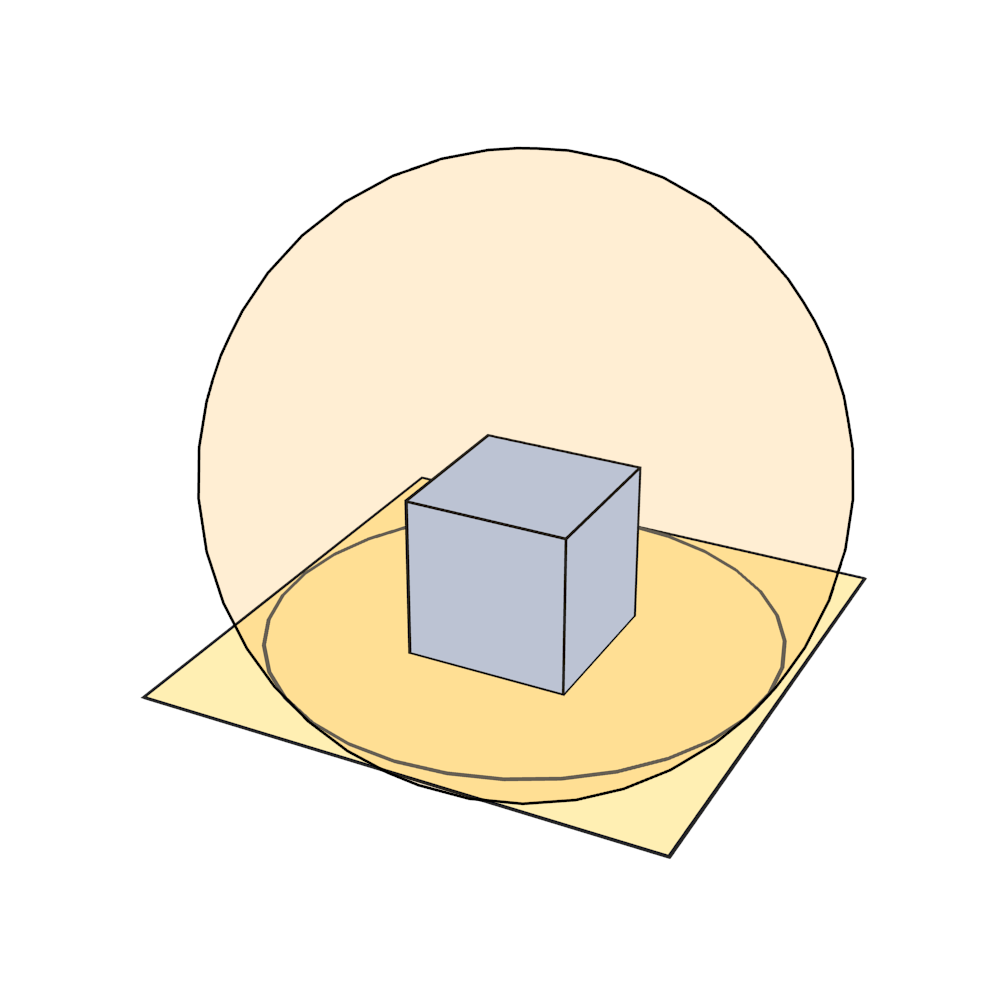
\includegraphics[width=\textwidth]{./img/raw/besluit-geom/scene.png}
  \caption{Simple scene.}
  \label{fig:vo-geometrie:0}
  \end{subfigure}%
  \begin{subfigure}[b]{0.249\textwidth}
    \centering
  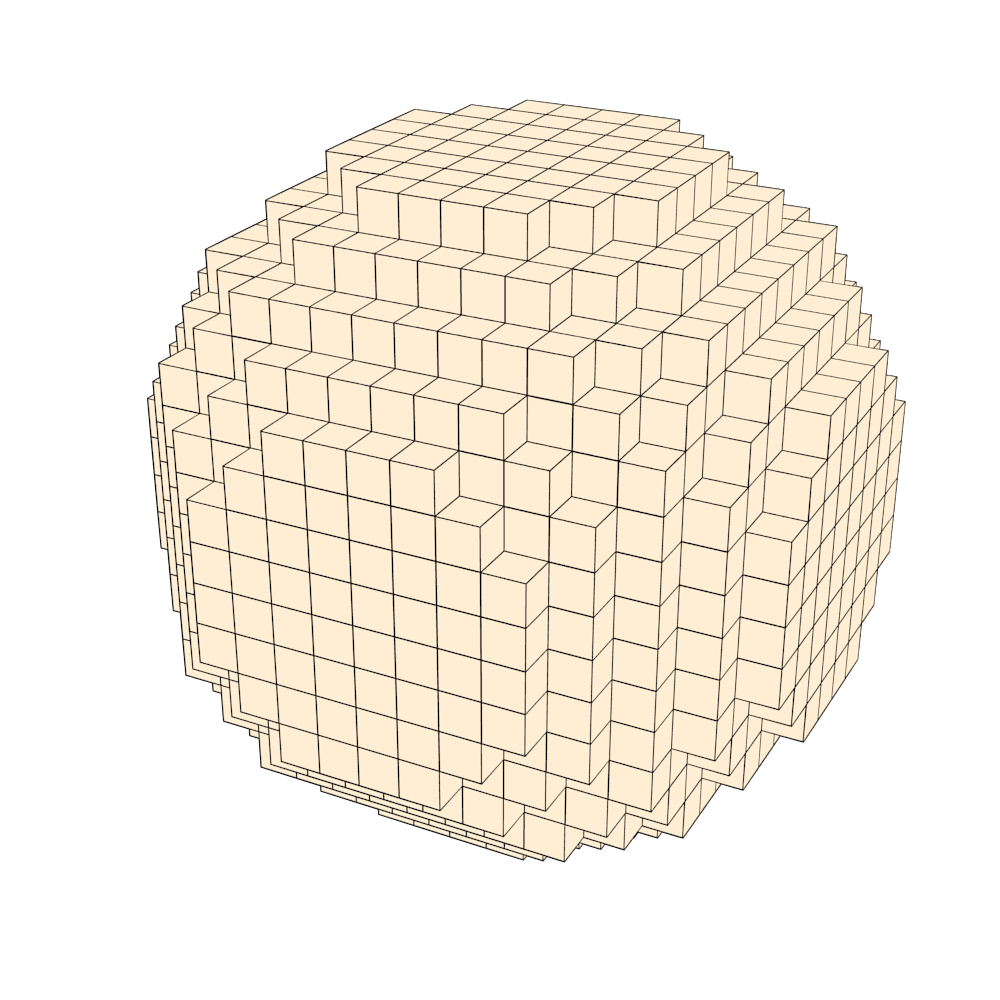
\includegraphics[width=\textwidth]{./img/raw/besluit-geom/light.png}
  \caption{Light nodes.}
  \label{fig:vo-subsets:1}
  \end{subfigure}\\
  \begin{subfigure}[b]{0.249\textwidth}
    \centering
  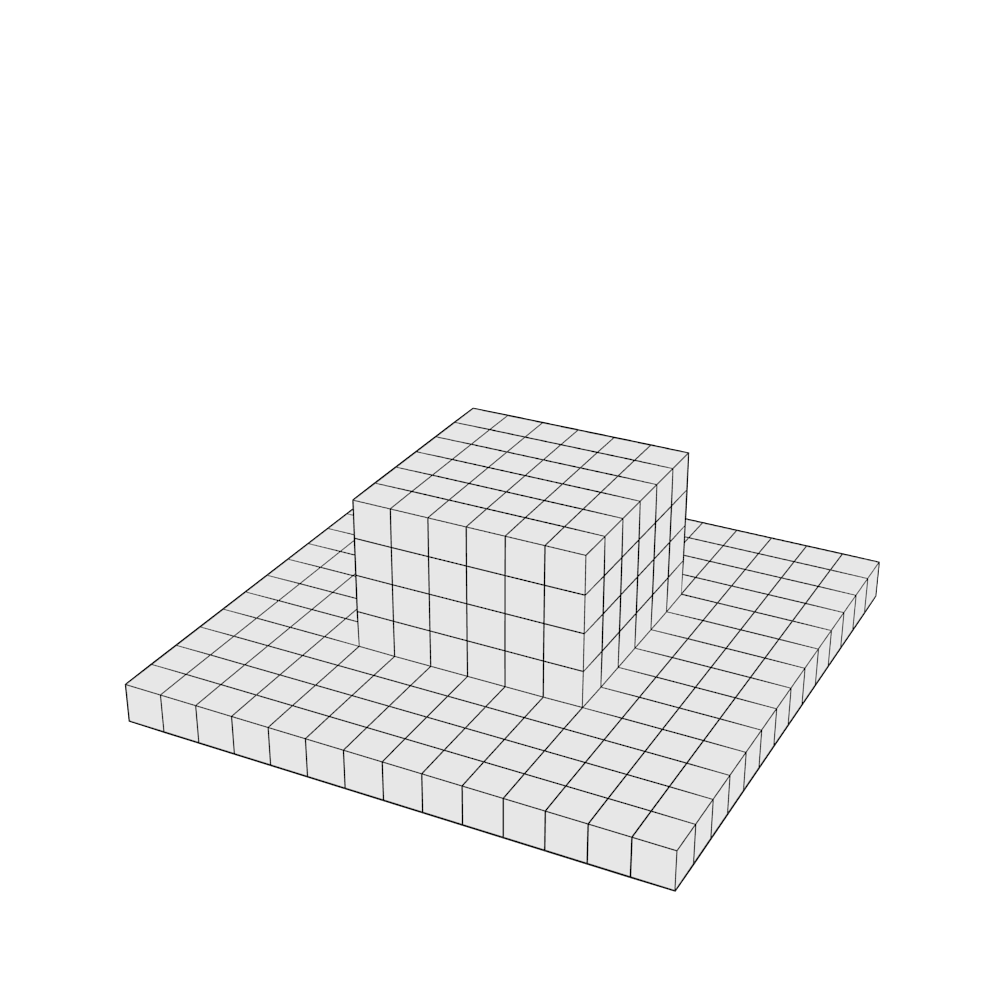
\includegraphics[width=\textwidth]{./img/raw/besluit-geom/geom.png}
  \caption{Geometry nodes.}
  \label{fig:vo-geometrie:0}
  \end{subfigure}%
  \begin{subfigure}[b]{0.249\textwidth}
    \centering
  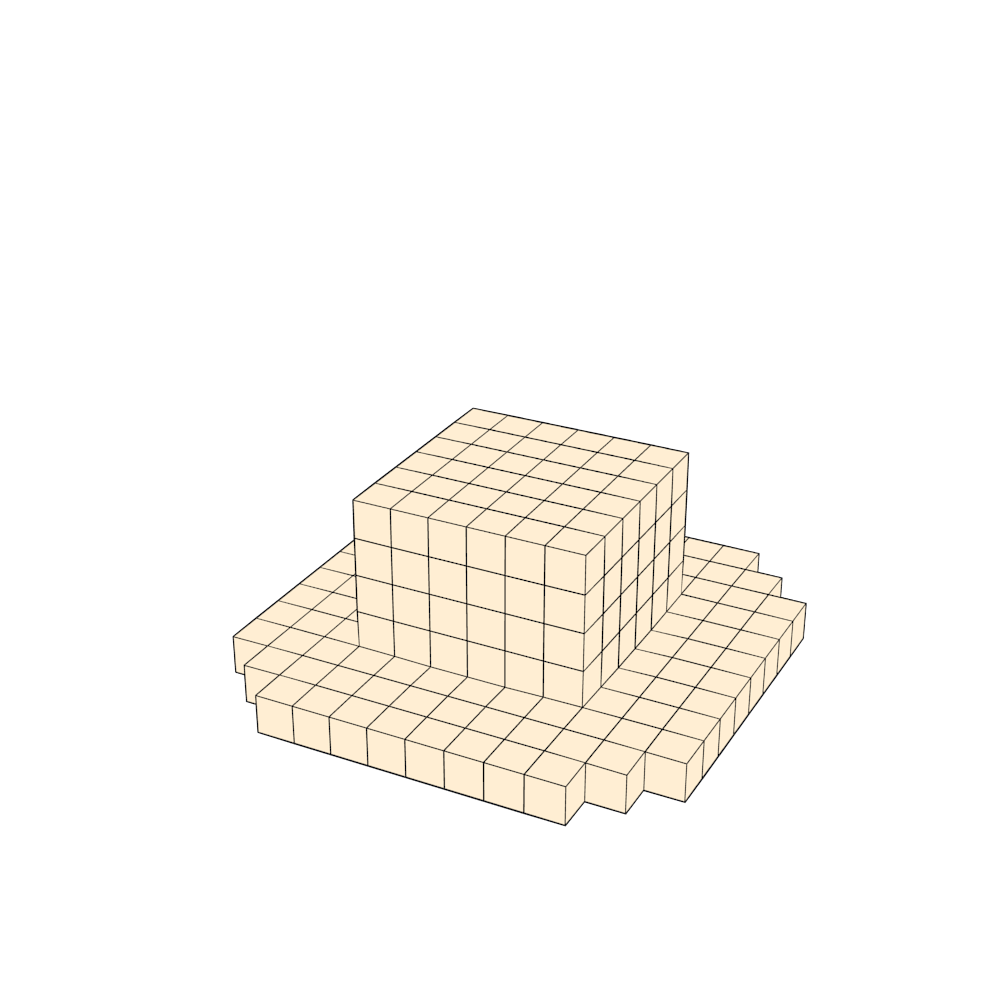
\includegraphics[width=\textwidth]{./img/raw/besluit-geom/comb.png}
  \caption{Light geometry nodes.}
  \label{fig:vo-subsets:1}
  \end{subfigure}
  \caption{Reduction of the number of nodes by excluding empty space.}
  \label{fig:vo-geometrie}
\end{figure}
